\documentclass[12pt,a4paper]{article}

% Quelques options d'encodage, de langues et de format du document
\usepackage[utf8]{inputenc}
\usepackage[T1]{fontenc}
\usepackage[english]{babel}
\usepackage[top=2cm, bottom=3cm, left=1.75cm, right=1.75cm]{geometry}
\usepackage{setspace}

\usepackage{graphicx} % Pour la commande "\includegraphics"
\usepackage[ % Modified parameters
    bookmarks,
    colorlinks,
    citecolor=black,
    urlcolor=blue,
    linkcolor=black,
    pdfpagemode=UseNone
]{hyperref} % Pour la commande "\url"

\pagenumbering{arabic}

% ------------------------------------------------------------------
% CITATION MANAGEMENT
% ------------------------------------------------------------------

% APA Style
\usepackage{cite}
\bibliographystyle{apalike}

\renewcommand\refname{Bibliography}

% Proper formatting and line breaking for URLs
\usepackage{url}

% Change "References" to "Bibliography"
\usepackage{etoolbox}
\patchcmd{\thebibliography}{\section*{\refname}}{\section*{Bibliography}}{}{}

% ------------------------------------------------------------------
% SUBFIGURE MANAGEMENT
% ------------------------------------------------------------------

\usepackage[caption=false]{subfig}
\usepackage{pgfplots}
\usepgfplotslibrary{groupplots}
\pgfplotsset{compat=1.18}
\usepackage{booktabs}

% ------------------------------------------------------------------
% COLORED TEXT MANAGEMENT
% ------------------------------------------------------------------

\usepackage{xcolor}
\usepackage{todonotes}
\setuptodonotes{inline=always}
\setlength {\marginparwidth }{2cm}

% ------------------------------------------------------------------
% CODE MANAGEMENT
% ------------------------------------------------------------------

\usepackage{listings}
\usepackage{cleveref}

% needs sheel escape activated
% --shell-escape
%\usetikzlibrary{external}
%\tikzexternalize[prefix=figures_tikz_compiled/]

\lstdefinelanguage{Cypher}{
    morekeywords={
        MATCH, RETURN, WHERE, CREATE, DELETE, SET, MERGE, DETACH,
        WITH, LIMIT, SKIP, ORDER, BY, DESC, ASC, OPTIONAL, CALL
    },
    sensitive=true,
    morecomment=[l]{//},
    morecomment=[s]{/*}{*/},
    morestring=[b]',
    morestring=[b]"
}

% Listing style for better readability
\lstset{
    language=Cypher,
    basicstyle=\ttfamily\small,
    keywordstyle=\color{blue},
    stringstyle=\color{orange},
    commentstyle=\color{gray},
    showstringspaces=false,
    numbers=left,
    numberstyle=\tiny,
    breaklines=true,
    frame=single
}


\newcommand{\modelministral}{Ministral-8B}
\newcommand{\modelalpaca}{Alpaca-7B}
\newcommand{\modeldeepseek}{R1-Distill-8B}


\begin{document}

\begin{center}
    \begin{tabular}{|p{0.2\textwidth}|p{0.75\textwidth}|}
        \hline
        {
            \vspace{0cm} % without it, bugs, don't know why?
            \centerline{
\includegraphics[width=\linewidth]{./images/tp-ipp}}
        }
        & {
            \vspace{0cm} % same here
            \centering
            \large
            {\hfill February, 2025}

            \vspace*{.5cm}
            \textbf{APM\_5AI29\_TP}

            \vspace*{.5cm}
            \setstretch{1.5}
            {\Large\textbf{Language Models and Structured Data}}

            \vspace*{.5cm}
            Final Project Report

            \vspace*{1cm}
        } \\
        \hline
    \end{tabular}
\end{center}

\noindent Acronym of the Team: AWESome\\
Names: Mochamad Ardiansyah Nurgaha; William Liaw; Eddie Groh; Sriraam Appakutti Palani

    {\centering\rule{\linewidth}{.5pt}}

\begin{center}
    \section*{Knowledge Graph Completion}
\end{center}

\todo{Maybe abstract?}

% ---------------------------------------------------------
%
% PROBLEM STATEMENT
%
% ---------------------------------------------------------

\section{Problem Statement}\label{sec:problem_statement}
\todo{Define precisely what we are doing (predicting head/tail or just the relation?). Maybe Include a small example to illustrate the problem? Should not be necessary}
\todo{Be mathematically rigierous}

% Knowledge Graph Completion (KGC) is a fundamental task in artificial intelligence aimed at addressing the inherent incompleteness of knowledge graphs (KGs). KGs represent real-world facts as structured triples of the form $(h, r, t)$, where $h$ (head entity) and $t$ (tail entity) are connected by a relation $r$. Despite their widespread use in search engines, recommendation systems, and question-answering applications, KGs suffer from missing information, necessitating the development of KGC techniques to predict missing elements and improve KG utility.

% ---------------------------------------------------------
%
% BACKGROUND
%
% ---------------------------------------------------------


\section{Background}\label{sec:background}
\todo{Disguise for related work, however it should not look like related work. What has to be done here is to QUICKLY introduce classical models, then go over to the distingsion we are going to draw which is fine tuning vs. pure promt engineering. This clear distingsion does not exist, but we will pretend}
\todo{Talk about Prompt engineering, speciaially KICGPT, throw in a couple of other papers for additional BaCkGrOuND and find a reason why we choose KICGPT}
\todo{Same for KoPA}
\todo{VERY BRIEF general comparison of approaches}

Early KGC research centered on triple-based models using embedding methods to represent entities and relations in a continuous vector space. TransE \cite{bordes2013translating} models relations as translation operations, while DistMult \cite{yang2014embedding} and ComplEx \cite{trouillon2016complex} apply tensor factorization, the latter extending to complex-valued embeddings.

Advancements introduced Graph Neural Networks (GNNs) \cite{schlichtkrull2018modeling} to refine entity representations by aggregating structural information. However, these models struggle with long-tail entities due to sparse connectivity, limiting predictive performance.

To overcome these limitations, text-based KGC leverages pre-trained language models (PLMs) to incorporate entity and relation descriptions. KG-BERT \cite{yao2019kgbert} reframes KGC as a classification problem, encoding triples as text for distinguishing valid from invalid ones. Despite effectiveness, these methods require extensive fine-tuning and high computational costs, restricting scalability.

Large language models (LLMs) have revolutionized KGC via in-context learning (ICL) and instruction tuning, enabling link prediction without explicit retraining. Unlike fixed-structure KG models, LLMs leverage broad internal knowledge for zero-shot and few-shot predictions. However, they face challenges like hallucination (factually incorrect outputs) and structural misalignment with KG schemas.

Two main strategies integrate LLMs into KGC: \textbf{Purely Prompt-Based Methods}, which leverage structured retrieval and in-context learning without modifying model parameters, and \textbf{Fine-Tuning-Based Methods}, which embed structured knowledge into the model through additional training. The former is efficient and adaptable but depends on well-designed retrieval mechanisms, while the latter enhances domain-specific reasoning at the cost of increased computational demands and dataset dependency.

Among purely prompt-based approaches, KICGPT \cite{wei2023kicgpt} exemplifies a retriever-integrated prompting strategy, where a traditional triple-based KGC model retrieves a ranked list of candidate entities, which is then refined by an LLM through Knowledge Prompts—an in-context learning technique encoding KG structure into prompts. Similarly, MPIKGC \cite{xu2024mpikgc} enhances description-based KGC models by querying LLMs to expand entity descriptions, improve relation understanding, and extract structural information, without modifying the LLM's parameters. These methods demonstrate that effective KGC can be achieved without fine-tuning, reducing computational costs while leveraging structured retrieval mechanisms.

Conversely, fine-tuning-based approaches modify LLM parameters to embed structured KG knowledge directly. KoPA \cite{qin2023kopa} introduces a Knowledge Prefix Adapter, mapping KG structural embeddings into the LLM's textual space via an adapter network, allowing structure-aware guidance during inference. DIFT \cite{liu2024dift} fine-tunes LLMs with discrimination instructions, refining the model's ability to select correct KG entities while mitigating grounding errors. KC-GenRe \cite{wang2024kcgenre} proposes a knowledge-constrained generative re-ranking method, leveraging LLM fine-tuning to improve entity ranking through structured guidance. Additionally, RPKGC \cite{khalil2024rpkgc} fine-tunes an LLM for relation prediction, training the model to infer plausible relations between entity pairs. These methods enhance reasoning capabilities at the expense of increased training complexity and resource requirements.

Given their distinct yet complementary methodologies, the remaining sections of this report will focus on KICGPT and KoPA, providing a detailed examination of their underlying principles, implementation details, and comparative advantages in leveraging LLMs for KGC.

% ---------------------------------------------------------
%
% METHODOLOGY
%
% ---------------------------------------------------------

\section{Methodology}\label{sec:methodology}
\todo{Introduce KICGPT metho as "prompt engie" maybe throw in a couple of formulas}
\todo{FANCY PICTURE OF ARCHITECTURE}
\todo{Extend or intro KoPA as "fine tuning"}
\todo{Another ultra fancy picture}
\todo{it might be hard to seperate this from the previous section, however it should be possible, if not we can also fuse them, but it might hinder readability since we keep jumping all over the place (cause other papers are required for background)}

In this project, we focus on link prediction task for knowledge graphs
(KGs). Given incomplete triple in a KG \((h, r, ?)\) or \((?, r, t)\),
the goal is to predict the missing entity, either it is head \(h\)
or tail \(t\), where \(h, t \in E\) and \(r \in R\), E denotes set of
entities, R denotes set of relations. The model that we used follows
KICGPT \cite{wei2023kicgpt} with modification on the LLM used.

\subsection{Architecture}
\label{sec:method:architecture}

\begin{figure}
    \centering
    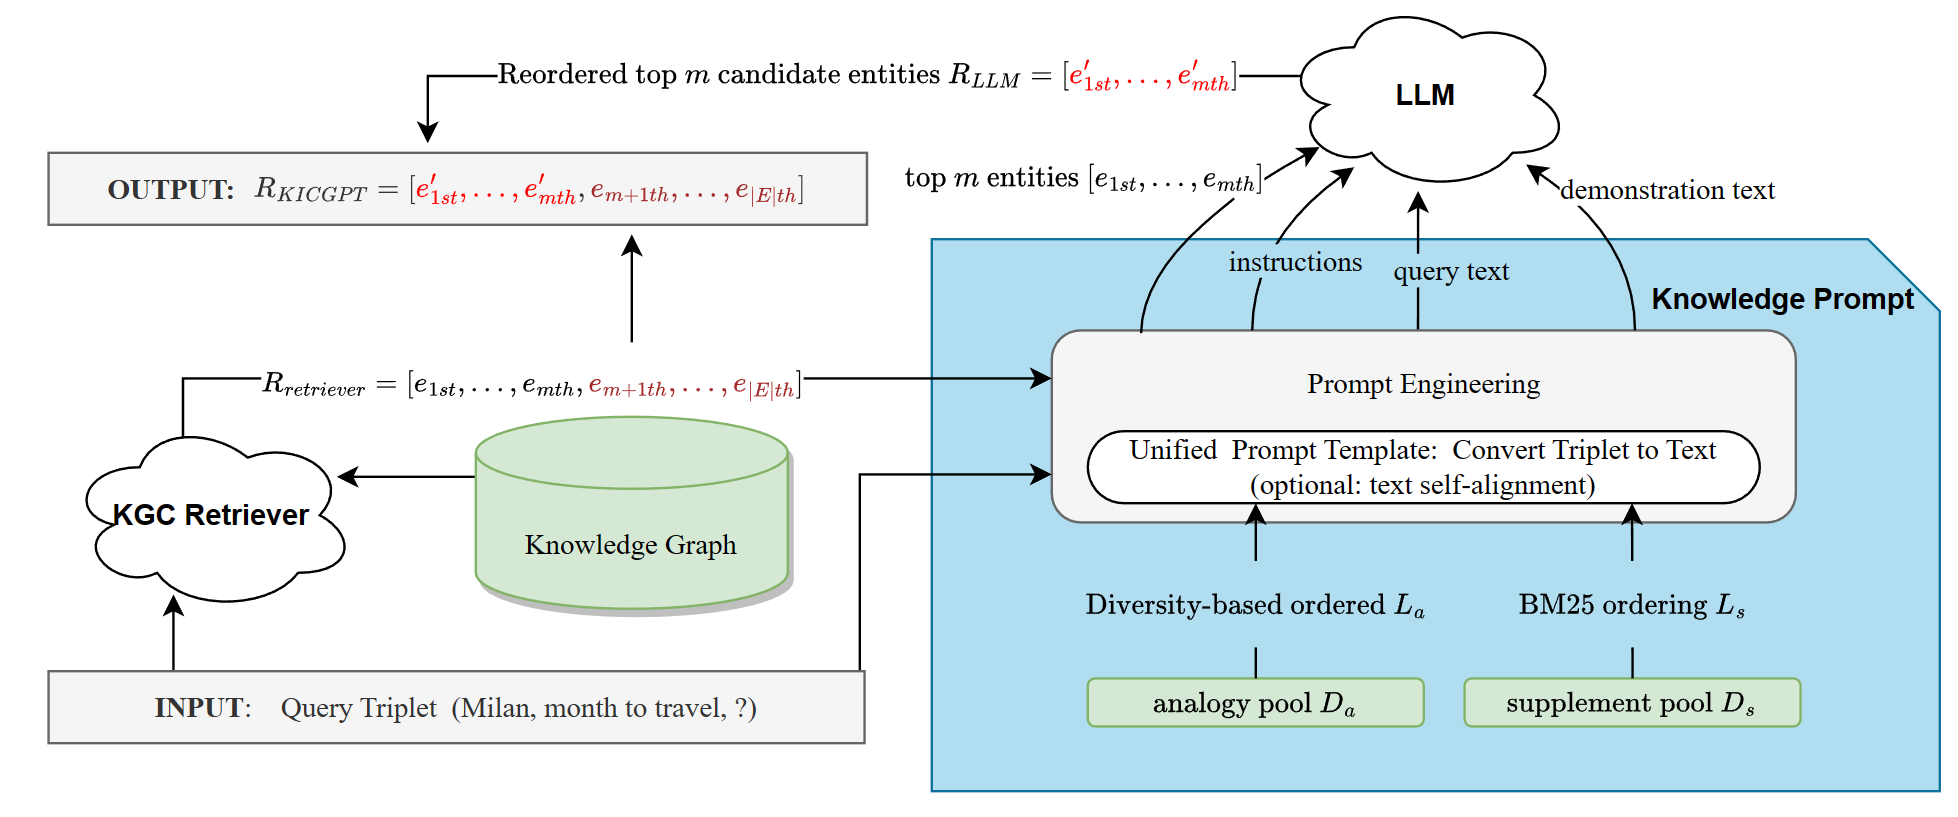
\includegraphics[width=0.8\textwidth]{figures/arc3.png}
    \caption{KICGPT Architecture \cite{wei2023kicgpt}}
    \label{fig:KICGPTarchitecture}
\end{figure}

KICGPT primarily covers three main components as can be seen in Figure
\ref{fig:KICGPTarchitecture}, which are a triple-based KGC retriever,
the Knowledge Prompt, and a LLM. For each query triple \((h, r, ?)\),
the KGC retriever retrieves the score of \((h, r, e)\) for each entity
\(e \in E\) in descending order
\(R_{retriever} = [e_1, e_2, ..., e_{|E|}]\).
Using prompt engineering in the Knowledge Prompt, LLM performs reranking
of the top \(m\) entities
\(R_{LLM} = [e^{'}_1, e^{'}_2, ..., e^{'}_m]\). Finally, KICGPT will
output final ranking of top m entities from the LLM and the rest of
the entities from the KGC retriever
\(R_{KICGPT} = [e^{'}_1, e^{'}_2, ..., e^{'}_m, e_{m+1}, ..., e_{|E|}]\)

\subsubsection{Knowledge Prompt}
Knowledge Prompt is introduced in KICGPT as in-context learning
strategy to provide context to the LLM by integrating part of the KG
into the demonstration. There are two pools of triples in the
demonstration, analogy pool \(D_a\) and supplement pool \(D_s\).
To help the LLM understand the query triple, the analogy pool contains
triples with the same relation \(r\) as the query \((h, r, ?)\),
\(D_a = \{(e^{'}, r, e^{"}) \in G_{train} \cup G_{valid} \mid e, e^{"} \in E\}\).
In addition, the supplement pool contains triples with one of its entity
(tail or head) is the same as the query's head \((h, r, ?)\),
\(D_s = \{(h, r, e^{'}) \in G_{train} \cup G_{valid} \mid r^{'} \in R, e^{'} \in E\} \cup
\{(e^{'}, r, h) \in G_{train} \cup G_{valid} \mid r^{'} \in R, e^{'} \in E\}\).
This is to provide additional information of the query's head to the LLM.

The ordering of the demonstration is important as it affects the LLM performance.
For the analogy pool, each entity starts with a zero counter.
A random triple from \(D_a\) is chosen first, increasing its entities'
counters by 1. Next, the triple with the lowest summed counter values
is selected, repeating until all triples are used. The final ordered
list is denoted \(L_a\). The supplement pool \(D_s\) provides additional context
for the query's head entity \(h\), prioritizing relevant demonstrations.
To achieve this, triples in \(D_s\) are ranked based on their BM25 scores,
which measure their textual similarity to the query. The final ordered list,
denoted \(L_s\), includes all triples from \(D_s\).

\subsubsection{Prompt Engineering}

To adapt structured triples into natural language input, KICGPT uses
a unified prompt template, ensuring consistent formatting for queries
and demonstrations. The interaction with the LLM follows a multi-round
process. First, the responsibility description stage clarifies the LLM's
role in ranking candidate answers. Next, in the question and demonstration
description stage, the query is presented along with an explanation of
two demonstration types: analogy-based and supplementary examples.

In the demonstration input stage, batches of demonstrations from the
analogy \(L_a\) and supplement \(L_s\) pools are provided, repeated
as much as the token limit allows to maximize knowledge inclusion.
Finally, during the final query and re-ranking stage, the LLM ranks
the top-m candidate entities, producing an ordered list \(R_{LLM}\),
which replaces the top-m results from the retriever to generate the
final answer.

% ---------------------------------------------------------
%
% EXPERIMENTS
%
% ---------------------------------------------------------

\section{Experiments}\label{sec:experiments}

\begin{figure}
    \centering
    \begin{tikzpicture}
        % Group plot configuration
        \begin{groupplot}[
            group style={
                group size=3 by 1,       % 3 plots in 1 row
                horizontal sep=0.3cm     % Adjust spacing between plots
            },
            width=0.38\textwidth,        % Maximized plot width
            ymode=log,                   % Log-scale y-axis for ALL plots
            xmin=0, xmax=3,              % Unified x-axis range
            ymin=1e-3, ymax=1,           % Unified y-axis range across all plots
            xlabel=Epoch,
            xtick distance=0.5,          % Uniform tick spacing
            ytick distance=10,           % Log-scale tick separation
            minor y tick num=9,          % Minor tick marks for readability
        ]

            %------------- Plot (a) Alpaca -----------------
            \nextgroupplot[
                title=Alpaca,
            % Hide y-axis labels for alignment
                ylabel=Loss
            ]
            \addplot[smooth, thick, blue]
            table[x=epoch, y=loss, col sep=space]
                {figures/raw-data/lora-Llama-2-7b-alpaca-cleaned-finetune.dat};

            \addplot[smooth, thick, cyan, dashed]
            table[x=epoch, y=grad-norm, col sep=space]
                {figures/raw-data/lora-Llama-2-7b-alpaca-cleaned-finetune.dat};


            %------------- Plot (b) DeepSeek ---------------
            \nextgroupplot[
                title=R1-Distill,
                yticklabels={,,}
            ]
            \addplot[smooth, thick, purple]
            table[x=epoch, y=loss, col sep=space]
                {figures/raw-data/lora-DeepSeek-R1-Distill-Llama-8B-finetune.dat};

            \addplot[smooth, thick, violet, dashed]
            table[x=epoch, y=grad-norm, col sep=space]
                {figures/raw-data/lora-DeepSeek-R1-Distill-Llama-8B-finetune.dat};

            %------------- Plot (c) Loss Comparison -------------
            \nextgroupplot[
                title=Loss Comparison,
                yticklabels={,,}   % Hide y-axis tick labels for uniform look
            ]
            \addplot[smooth, thick, purple]
            table[x=epoch, y=loss, col sep=space]
                {figures/raw-data/lora-DeepSeek-R1-Distill-Llama-8B-finetune.dat};

            \addplot[smooth, thick, blue]
            table[x=epoch, y=loss, col sep=space]
                {figures/raw-data/lora-Llama-2-7b-alpaca-cleaned-finetune.dat};

        \end{groupplot}
    \end{tikzpicture}

    % Description of colors with more spacing in legend
    \vspace{0.2cm}
    {\centering
        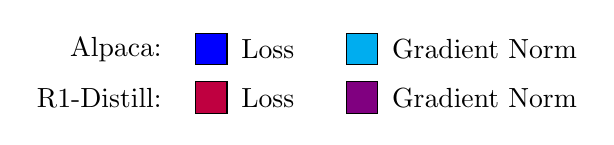
\begin{tikzpicture}
            \node[draw, fill=blue, minimum width=0.4cm, minimum height=0.4cm] (A) {};
            \node[left=0.3cm of A] {Alpaca:};
            \node[right=0.05cm of A] {Loss};

            \node[draw, fill=cyan, minimum width=0.4cm, minimum height=0.4cm, right=1.5cm of A] (B) {};
            \node[right=0.05cm of B] {Gradient Norm};

            \node[draw, fill=purple, minimum width=0.4cm, minimum height=0.4cm, below=0.2cm of A] (C) {};
            \node[left=0.3cm of C] {R1-Distill:};
            \node[right=0.05cm of C] {Loss};

            \node[draw, fill=violet, minimum width=0.4cm, minimum height=0.4cm, right=1.5cm of C] (D) {};
            \node[right=0.05cm of D] {Gradient Norm};
        \end{tikzpicture}
    }

    \caption{Training performance comparison of DeepSeek and Alpaca models.
        (a) and (b) show loss and gradient norm trends separately for each model,
        while (c) compares both losses for direct convergence analysis. \todo{fix description}}
    \label{fig:training_comparison}
\end{figure}


\todo{Maybe shortly explain dataset?}
\todo{maybe QUICKLY intro metrics, however should be known already}

\subsection{Concise Model Summaries}

We use three models for our experiments:
Alpaca-7B~\cite{taori2023stanford} is a fine-tuned LLaMA 7B model designed for instruction-following tasks, trained on 52,000 examples generated via OpenAI’s text-davinci-003.
Ministral-8B-Instruct-2410~\cite{mistralai2024ministral8b} is an 8-billion-parameter model fine-tuned for instruction tasks, featuring a 128k context window and multilingual support, outperforming similar-sized models.
Compared to Alpaca, Ministral-8B benefits from a larger model size, an extended context window, and broader multilingual capabilities.
DeepSeek-R1-Distill-Llama-8B~\cite{deepseekai2025deepseekr1distillllama8b} is an 8-billion-parameter model distilled from DeepSeek-R1~\cite{guo2025deepseek}, focusing on reasoning and problem-solving, particularly excelling in math and code tasks.

All experiments were conducted on a system equipped with an NVIDIA RTX A5000 GPU with 24 GiB of VRAM, paired with an Intel Xeon W-1270P CPU running at 3.80 GHz and 64 GB of RAM.

\todo{Performance of KICGPT}

Following the procedure outlined in~\cref{sec:methodology}, we finedtuned \modelalpaca on CoDeX~\cite{safavi2020codex} dataset.
This process took 10 Hours and 12 Minutes, with very consistent

\todo{very unhappy with this, we need to write somethign like this}
Following the procedure outlined in~\cref{sec:methodology}, we fine-tuned \modelalpaca on the CoDeX~\cite{safavi2020codex} dataset.
This process took 10 hours and 12 minutes, with the model converging as expected.
The training loss, shown in the leftmost plot of \cref{fig:training_comparison}, follows a bit noisy downward trend, while the gradient norm exhibits significant fluctuations but also trends downards over time.

Similarly, \modeldeepseek was fine-tuned under the same setup, with its training loss shown in the middle plot of \cref{fig:training_comparison}. The loss curve behaves similarly to \modelalpaca, confirming stable convergence, though the gradient norm remains similarly volatile throughout training.
The decreasing trend in gradient norm suggests that while updates remain unstable at each step, their overall magnitude diminishes as training progresses, indicating a gradual refinement of the optimization process.

The final comparison, shown in the rightmost plot of \cref{fig:training_comparison}, demonstrates that both models achieve nearly identical loss trajectories.
So we would expect them to perform similarly.

\todo{eval of deepseek and alpacca}


% ---------------------------------------------------------
%
% DISCUSSION
%
% ---------------------------------------------------------

\section{Discussion}\label{sec:discussion}
\todo{TBD, only do if there is actual deeper meaning otherwise fuse with experiments}

\todo{Interpret the results in a deeper way:
- Why did certain methods do better?
- Mention any error analysis or interesting observations.
}

% ---------------------------------------------------------
%
% CONCLUSION
%
% ---------------------------------------------------------

\section{Conclusion and Future Work}\label{sec:conclusion-and-future-work}
\todo{TBD otherwise leave out}
\todo{Summarize the key findings and how they link back to your problem statement. Suggest improvements or next steps (e.g., new dataset, advanced fusion technique, or GNN-based approach). Highlight what you learned and what remains challenging.}

\bibliography{main}

\end{document}
